 \documentclass[withoutpreface,bwprint]{cumcmthesis} %去掉封面与编号页,电子版提交的时候使用。


\usepackage[framemethod=TikZ]{mdframed}
\usepackage{url}   % 网页链接
\usepackage{subcaption} % 子标题
\usepackage{longtable}
\usepackage{graphicx}
\usepackage{subcaption} 
\title{基于线性规划的农作物种植问题}
\tihao{A}
\baominghao{xxxx}
\schoolname{XX大学}
\membera{ }
\memberb{ }
\memberc{ }
\supervisor{ }
\yearinput{2023}
\monthinput{09}
\dayinput{04}
\graphicspath{{figures/}}  
\begin{document}

 \maketitle
 \begin{abstract}
 	
 	在乡村发展中,充分利用有限的耕地资源,因地制宜地发展有机种植产业,对实现经济的可持续发展具有重要的现实意义。选择适宜的农作物并优化种植策略,有助于提高生产效益,方便田间管理,同时减少各种不确定因素带来的种植风险。在此背景下,研究乡村2024$\sim$2030年的农作物种植方案显得尤为重要。
 	
	\textbf{针对问题一},主要解决在各情况相对于与2023年保持稳定的情况下,针对两种不同情况,分别给出2024~2030年农作物的最优种植方案。本研究先对数据进行分析和预处理,从中提取了2023年的各指标,然后以利润为目标函数,农作物土地面积限制,作物的土地适宜性的限制,单季农作物种植限制,连续重茬种植限制,优化耕种作业和田间管理,改善土壤养分状况为约束建立\textbf{混合整数规划模型}。将最优种植方案分为一年一期,共七期,为求解复杂的线性优化问题,使用MATLAB编写\textbf{遗传算法(GA)}代码求解模型,最终算出了2024至2030年间在情况一下的总利润为\textbf{2.0251千万},情况二下的总利润为\textbf{4.2132千万},并给出相应的土地分配方案,具体方案见目录。
	
	\textbf{针对问题二},主要解决综合考虑各种农作物的未来的不确定性及其风险的影响下,在问题一的基础下给出2024~2030年农作物的最优种植方案。本研究通过构建扰动模型和运用蒙特卡洛模拟来分析农作物生产中的不确定性,以评估不同因素对种植结果的影响。由于气候变化、市场波动等因素使得农作物的预期销售量、亩产量、种植成本和销售价格存在一定程度的年际波动,最后进行扰动处理,预测未来数据的动态变化。再结合问题一的混合整数规划模型,最终算出了2024至2030年总利润为\textbf{1.9493千万},并给出相应的土地分配方案。
	
	\textbf{针对问题三},主要解决农作物的可替代性与互补性,分析了预期销售量、销售价格与种植成本之间的相关性。首先,通过\textbf{k-means聚类}将价格相似的作物分组,以识别它们的替代性关系。其次,采用对数函数拟合预期销售量、销售价格和种植成本的数据,结果表明预期销售量与销售价格存在负相关性,而销售价格与种植成本有正相关性。销售价格和种植成本之间的相关性较弱可忽略。最后,结合模拟数据,结合\textbf{多目标遗传算法}
\textbf{	NSGA-II},依据作物成本与售价的变化进行调整,提出了具体的调整步骤。结果表明,在市场因素的波动下,作物的替代性与数据关联性对调整策略有显著影响。
\keywords{\quad 混合整数规划模型,\quad 遗传算法(GA)\quad 扰动模型 \quad k-means聚类}\quad NSGA-II
\end{abstract}


%\tableofcontents

%\newpage

\section{问题背景}
在乡村发展中,充分利用有限的耕地资源,因地制宜地发展有机种植产业,对实现经济的可持续发展具有重要的现实意义。选择适宜的农作物并优化种植策略,有助于提高生产效益,方便田间管理,同时减少各种不确定因素带来的种植风险。

在此背景下,研究乡村2024$\sim$2030年的农作物种植方案显得尤为重要。针对未来农作物的销售量、种植成本、亩产量和销售价格的稳定性,以及各种不确定性因素,建立数学模型将有助于制定出科学合理的种植策略。

\section{问题重述}
        \subsection{问题一}
        假设未来农作物的销售量、种植成本、亩产量和销售价格保持稳定。如果某作物的产量超过预期销售量,超出部分无法销售。请为乡村制定2024~2030年的最优种植方案,分别考虑以下两种情况,并填写在相应文件中:
        \begin{enumerate}
        	\item 超出部分滞销。
        	\item 超出部分按50$\%$降价出售。
        	
        \end{enumerate}
        \subsection{问题二}
        考虑农作物的销售量、亩产量、种植成本和价格的不确定性,为乡村制定2024$\sim$2030年的最优种植方案,并填写在指定文件中。
        \subsection{问题三}
        在问题2的基础上,综合考虑农作物之间的替代性和互补性,制定乡村2024$\sim$2030年的最优种植策略,并与问题2的结果进行比较分析。
        
\section{问题分析}
	\subsection{问题一}
	首先,以未来种植的作物种类和种植面积为决策变量,建立一个利润最大化的线性规划模型,并通过设置约束条件(如可用土地面积和各作物的最大种植量)确保种植方案的可行性。在考虑滞销情况下,更新目标函数,将那些超过预期销售量的作物按降价出售的收入纳入分析。最终,通过求解线性规划模型,得到最优种植面积分配,从而有效减少滞销风险并提高整体经济效益。
	\subsection{问题二}
	在确定未来种植方案的基础上,以作物种植面积和销售量为决策变量,建立最大化经济收益的优化模型。该模型需考虑市场的不确定性因素,例如不同作物的年增长率和销售价格波动。使用蒙特卡洛模拟方法进行多次随机抽样,评估不同种植组合的预期收益,并分析作物间的相互影响,以确定最佳种植方案。通过这种方法,能够在不确定的市场环境中,选择出既能最大化收益又能有效降低风险的种植策略。
	\subsection{问题三}
	
	在问题二的基础上,进一步考虑作物的可替代性与互补性,建立优化模型。优化目标是提高整体经济效益及降低潜在风险。模型中评估各作物的种植面积波动对总收益的影响,并结合不同作物之间的关系进行综合分析。采用基于动态规划方法进行求解,确保在复杂的市场环境下,能够找到最优的种植组合与策略,以实现收益最大化和风险最小化。
\section{模型的假设}
\begin{enumerate}
	\item 假定各种农作物未来的预期销售量、种植成本、亩产量和销售价格相对于 2023 年保持稳定
	\item 每季种植的农作物在当季销售

	\item 根据查询文献可知,寒冷的季节,许多农作物难以生长,菌类因为不依赖阳光进行光合作用,而通过分解有机物质来获取营养,这使得它们能够在低温环境中茁壮成长。而第二季恰为9月到次年4月,因此我们设定菌类只在每年的第二季种植。
	
	\item  2023年农作物的生产量为2024年农作物的预销量
\end{enumerate}
\section{符号说明}

\begin{table}[H]
		\caption{符号说明}\label{tab:001} \centering
	\begin{tabular}{cc}
		\toprule[1.5pt]
		$X_{ijt}^{k}$ & $k$年$t\text{季度时}i\text{种作物在}j\text{块地的种植面积}$ \\ $Y_{ijt}^{k}$&$k$年 $t\text{季度时}i\text{作物在}j\text{块地是否种植}$ \\
		$Area_j$ &$ j\text{块地的面积}$\\ $Price_{it}^{k}$&$k$年 $t\text{季度时}i\text{种农作物的每亩的售价}$\\
		$Product_{ijt}^{k}$ &$k$年 $t\text{季度时}i\text{种作物在}j\text{块地的亩产量}$ \\ $PSale_{ijt}^{k}$& $k$年$t\text{季度时}i\text{种作物在}j\text{块地的预期销量}$\\
		$Cost_{ijt}^{k}$ &$k$年$ t\text{季度时}i\text{种农作物在}j\text{块地的成本}$ \\$P$ & 利润函数 \\
		\bottomrule[1.5pt]
	\end{tabular}
	 %\begin{tablenotes}
	%	\footnotesize
	%	\item[*] *\textbf{未加特别说明, $i$=1,2, $\cdots $,41   %j$=1,$\cdots$ ,54  $t$=1,$\cdots$ ,6}
	%\end{tablenotes}
\end{table}

\section{问题一的模型建立与求解}
\subsection{数据预处理}
由于二表中并未给出明确的预期销售量,通过调查文献我们得到农产品滞销率在0.003左右,因此我们将\textbf{2024$\sim$2030} 年农作物的预期销售量近似为2023年农产品产出量。
\subsection{最优种植方案目标规划模型}
\subsubsection{模型分析}
本题通过构建目标规划模型,合理分配作物种植策略,在不违反题目所约束条件下,求解出不同滞销处理方案下,利\textbf{润最大化}种植方案。
\subsubsection{模型建立}
我们将最优种植方案划分为三年一期,共两期。为了便于计算,我们规定一年有两季,一期有六季,且以季作为计算单位以便于求解。

根据不同处理滞销农产品方案,我们构建了两种目标函数,同时引入\textbf{决策变量}$X_{ijt}$和$Y_{ijt}$,二者满足以下初始约束:
\begin{equation}
	\begin{cases}
		X_{ijt}\geqslant 0\\
		Y_{ijt}=1\text{或}Y_{ijt}=0\\
	\end{cases}
\end{equation}

对于\textbf{第一种处理方}案:超过部分滞销,造成浪费,我们构建如下目标函数:
\begin{equation}
\max \quad P=\sum_{k=1}^7{\sum_{t=1}^2{\sum_{j=1}^{54}{\sum_{i=1}^{41}{{PSale^k}_{ijt}\times {Price^k}_{it}-{Cost^k}_{ijt}}\times {X^k}_{ijt}\times {Y^k}_{ijt}}}}
\end{equation}

对于\textbf{第}\textbf{二种处理方案}:超过部分按 2023 年销售价格的 50$\%$降价出售,我们构建如如下目标函数:
\begin{equation}
	\begin{split}
\max \quad P=\sum_{k=1}^7{\sum_{t=1}^2{\sum_{j=1}^{54}{\sum_{i=1}^{41}{(}}}}{PSale^k}_{ijt}\times {Price^k}_{it}+0.5\times ({X^k}_{ijt}\times {Y^k}_{ijt}-{PSale^k}_{ijt})\times {Price^k}_{it}
\\
-{Cost^k}_{ijt}\times {X^k}_{ijt}\times {Y^k}_{ijt})
	\end{split}
\end{equation}

同时,根据题目的要求,我们对这些决策变量加以约束

\begin{itemize}
	\item \textbf{作物的土地适宜性的限制}
\end{itemize}

	由题可得,我们有如下约束条件:
	
	1.平旱
	地、梯田和山坡地适宜每年种植\textbf{一季粮食类作物}
	
	\begin{equation}
		\sum_{i=17}^{41}{\sum_{j=1}^{26}{\sum_{k=1}^7{\sum_{t=1}^2{{Y^k_{ijt}}=0}}}}
	\end{equation}
	
	2.水浇地适宜每年种植一季水稻或两季蔬菜
	
	
	\begin{equation}
		\sum_{i=1}^{15}{\sum_{j=27}^{34}{\sum_{k=1}^7{\sum_{t=1}^2{{Y^k_{ijt}}=0}}}}
	\end{equation}
	
	3.普通大棚适宜每年种植一季蔬
	菜和一季食用菌
	
	\begin{equation}
		\sum_{i=1}^{15}{\sum_{j=35}^{54}{\sum_{k=1}^7{\sum_{t=1}^2{{Y^k}_{ijt}=0}}}}
	\end{equation}
	
	4.智慧大棚适宜每年种植两季蔬菜
	\begin{equation}
			\begin{split}
				\sum_{i=1}^{16}{\sum_{j=51}^{54}{\sum_{k=1}^7{\sum_{t=1}^2{{Y^k}_{ijt}=0}}}}
				\\
				\sum_{i=38}^{41}{\sum_{j=51}^{54}{\sum_{k=1}^7{\sum_{t=1}^2{{Y^k}_{ijt}=0}}}}
				\\
			\end{split}
	\end{equation}
	
	对于土地适宜性对作物生长的限制,其描述的是对于任意一块地,对于不适宜这块地的作物不应该进行种植,也就是不适宜这块地的作物的所有季度的0-1变量加总应为0。
	
	\begin{itemize}
		\item \textbf{单季农作物种植限制}
	\end{itemize}
	
	对于单季度与双季度种植限制,考虑到部分作物一次种植周期长达两个季度,我们有如下约束
	\begin{equation}
		\begin{split}
			\sum_{i=1}^{16}{\sum_{j=1}^{26}{\sum_{k=1}^7{{Y^k}_{ij2}=0}}}
			\\
			\sum_{j=27}^{34}{\sum_{k=1}^7{{Y^k}_{1jt}=0}}
			\\
		\end{split}
	\end{equation}
	
	其描述的是,对于任意一年第二季度的0-1变量等于0。也就是说,对于单季度种植作物及其土地,我们规定只得在第一季度种植,同时也限定了在一年中单季度种植作物只得种植一次。
	
	\begin{itemize}
	\item \textbf{连续重茬种植限制}
	\end{itemize}
	
	对于连续重茬种植限制,我们规定连续的两季度之间不得种植同一种类作物,有如下约束条件:
	\begin{equation}
		{Y^k}_{ijt}+{Y^k}_{ij\left( t+1 \right)}\le 1\left( \text{其中}1\leqslant i\leqslant 5 \right)  
	\end{equation}
	其描述的是,在任意连续的两个季度之间,不应该出现重复的作物,且对于单季度土地而言,任意连续的两个季度应为第一季度与第三季度以此为例。
	\begin{itemize}
	\item \textbf{优化耕种作业和田间管理}
	\end{itemize}
	
	为了便于耕种作业和田间管理,我们设定在单个地块(除大棚外)中种植面积最低为该土地面积的20$\%$:
	
	\begin{equation}
		{X^k}_{ijt}\times {Y^k}_{ijt}\geqslant 0.2\times Area_j\times {Y^k}_{ijt}
	\end{equation}
	\begin{itemize}
	\item \textbf{改善土壤养分状况}
	\end{itemize}
	
	为了满足三年内至少种植一次大豆,使土地富含豆类作物根菌的土壤以有利于其他作物,有如下约束模型:
	\begin{equation}
	\sum_{t=n}^{n+5}{{Y^k}_{ijt}}\geqslant 1(n=1,2\cdots ,9)
	\end{equation}
	
	其描述的是在三年中的任意一次季度中,至少有一个季度种植豆类作物。且因为我们划分三年为一期计划,在下期计划中也应当进行一次以上约束。
	
	
	\begin{itemize}
		\item \textbf{预期售量与产量的约束(第一种处理方案)}
	\end{itemize}
	
	此时,我们假设预计售量是大于等于产量的,故约束如下:
	\begin{equation}
		{X^k}_{ijt}\times {Y^k}_{ijt}\times {Product^k}_{ijt}\leqslant {PSale^k}_{ijt}\times {Y^k}_{ijt}
	\end{equation}

\begin{itemize}
	\item \textbf{预期售量与产量的约束(第二种处理方案)}
\end{itemize}
	
此时,我们假设预计售量是小于等于产量的,故约束如下:
\begin{equation}
	{X^k}_{ijt}\times {Y^k}_{ijt}\times {Product^k}_{ijt}\geqslant {PSale^k}_{ijt}\times {Y^k}_{ijt}
\end{equation}
\subsection{模型求解}

建立起最优种植方案目标规划模型后,这是一个以三维矩阵为优化变量的复杂线性优化问题,运用普通lingo等软件难以求解。因此我们采用智能优化算法,即遗传算法(GA)对其进行优化仿真,并从时间复杂性、空间复杂性和收敛性等角度进行对比分析,最终得到最优配时方案。遗传算法(GA)具体流程如下图所示:


\begin{figure}[H]
	\caption{遗传算法流程图}
	\centering
	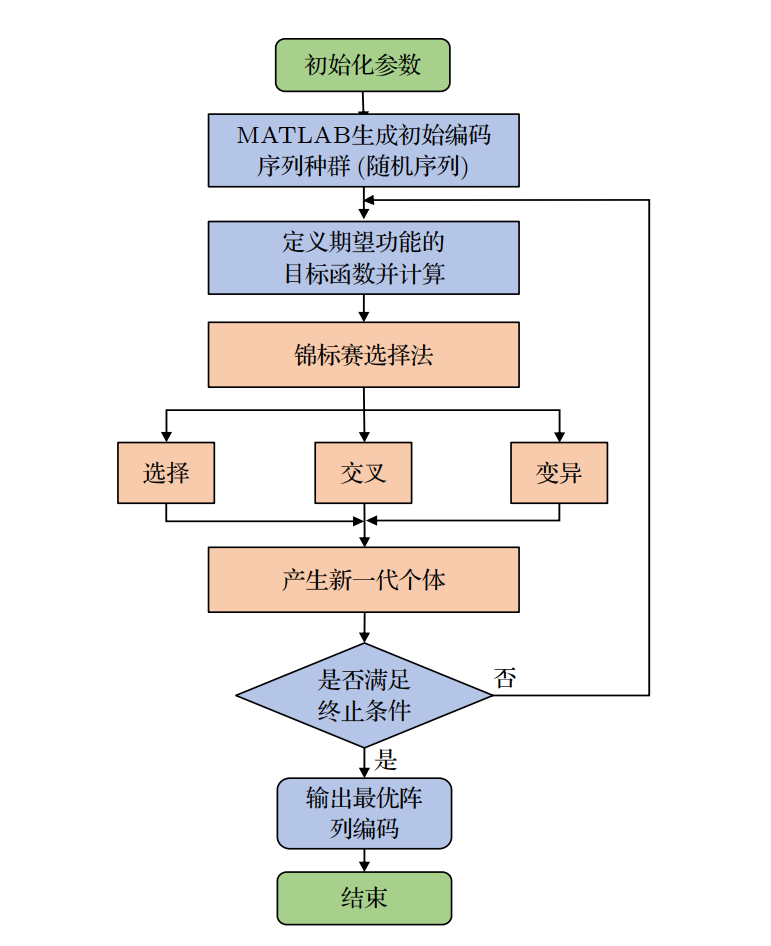
\includegraphics[width=0.5\linewidth]{figures/图片1}
\end{figure}

采用 MATLAB优化工具箱,对两种方案分别进行遗传算法优化,仿真过程需要的控制参数设置如下:两种算法的初始种群大小$I$均100,最大进化代数为50,遗传算法交叉率$P_c$均为0.8,变异率$P_m$均为  0.01,计算随机种群比例参数$r$时,$r_0 $取 0.1,$d$ 取 0.1;在算法参数设置不变的情况下,独立运行20次,取其最高。

两个方案各年的利润如下图所示,具体利润和土地分配见附录以及附件:

\begin{figure}[H]
	\centering
	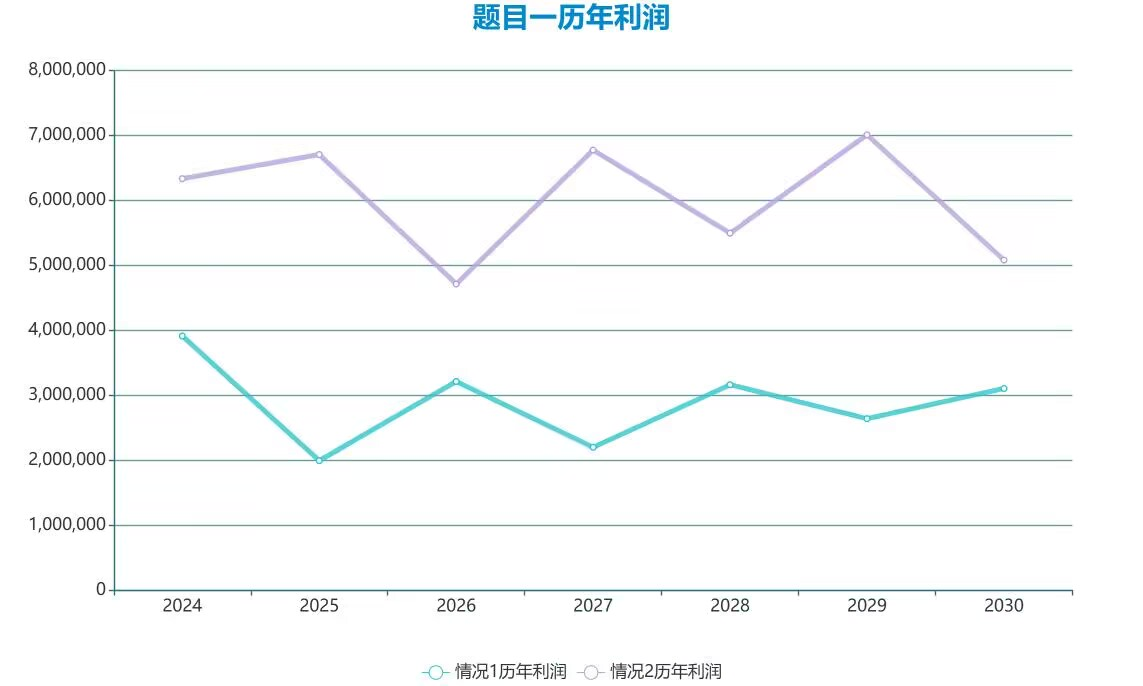
\includegraphics[width=0.8\linewidth]{figures/wentiyi}
\end{figure}


情况二由于超出预销量部分有额外售价,故理论上利润应高于情况一,如上图所示,情况二的利润显著高于情况一的利润,该情况检验了我们模型的正确性。同时求得情况一下的总利润为\textbf{2.0251千万},情况二下的总利润为\textbf{4.2132千万}
\section{问题二的模型建立和求解}
\subsection{扰动模型构建}

由于各种农作物的预期销售量、亩产量、种植成本和销售价格受气候,市场等因素的而产生的不确定性影响,在每年都会产生一定程度的波动,因此我们对此构建波动模型,对农作物的各项数据每年按题目所给数据进行调调整。

\subsubsection{蒙特卡洛模拟}

蒙特卡洛模拟可以基于变量的特定分布进行系统性的随机抽样模拟,当模拟次数足够多时,结果将逼近真实地数值。本文将这种方法引入于农作物各项数据中所涉未来值的预测。

由题意得,以2023年为基年,针对每一年的各项数据通过matlab蒙特卡洛模拟,进行扰动处理,对于点数据,我们采用正态分布$N(0,\frac{1}{600})$以期模拟增长率或下降率动态波动。

预期销售量:小麦和玉米预期销售量平均年增长率介于5\%$\sim$10\%,其他农作物每年的预期销售量大约有±5\%的变化。

\begin{equation}
	PSale^{k+1}_{ijt}=(1\pm5\times rand)\times PSale^{k+1}_{ijt}(i\ne 6,7)(rand\in[0,1])
\end{equation}

\begin{equation}
	PSale^{k+1}_{ijt}=(1.05+0.05\times rand)\times PSale^{k+1}_{ijt}(i= 6,7)(rand\in[0,1])
\end{equation}

亩产量:农作物的亩产量每年会有±10\%的变化。

\begin{equation}
	Prouduct^{k+1}_{ijt}=(0.9+rand\times 0.2)\times Prouduct^{k}_{ijt}(rand\in[0,1])
\end{equation}
 
种植成本:农作物的种植成本平均每年增长5\%左右。

\begin{equation}
	Cost^{k+1}_{ijt}=	(1+rand\times 0.05)(Cost^{k}_{ijt})(rand\in[0,1])
\end{equation}

销售价格:蔬菜类作物的销售价格有增长的趋势,平均每年增长5\%左右,食用菌的销售价格每年可下降1\%$\sim$5\%,但羊肚菌的销售价格每年下降幅度为5\%。

基于问题一中的自然约束,我们综合上述约束条件,求解如下目标函数:

\begin{equation}
	\max \quad P=\sum_{k=1}^7{\sum_{t=1}^2{\sum_{j=1}^{54}{\sum_{i=1}^{41}{{PSale^k}_{ijt}\times {Price^k}_{it}-{Cost^k}_{ijt}}\times {X^k}_{ijt}\times {Y^k}_{ijt}}}}
\end{equation}



通过计算方差,我们可以发现扰动后的的方差为4.0797E+11明显小于1.9843E+11的方差。这一发现表明,不确定性在种植过程中扮演了重要角色,并对种植效果产生了显著影响。这种不确定性可能是由各种潜在风险因素造成的,如气候剧烈变化、土壤条件的不均匀性、病虫害的爆发等。因此,潜在的种植风险确实存在,需要引起高度重视。为了优化种植策略和提高作物产量,应当采取措施来减少这些不确定性,改进种植环境管理和风险预测,以保障种植活动的稳定性和可持性。
\section{问题三的模型建立和求解}
\subsection{农作物的可替代性和互补性}

在微观经济学中,替代品和互补品是描述商品和服务之间相互关系的重要概念:

\textbf{替代品}:替代品是指在功能、用途或满足消费者需求方面相似的商品或服务,消费者可以互相替代使用这些商品或服务。

当一种商品的价格上升时,消费者可能会转向购买其替代品,因为替代品相对变得更便宜。替代品需求通常呈现负相关性,即一种商品的需求增加,其替代品的需求可能会减少。

\textbf{互补品}:互补品是指在消费时一起使用才能发挥最大效用的商品或服务,它们通常一起被购买和使用。在现实生活中,农产品之间的互补关系是较弱的,并没有说两种农产品之间一起使用能够显著增加效用,因此在本文中不考虑农产品的互补关系。
\subsubsection{k-mean聚类}

根据微观经济学中替代品与互补品的概念,我们发现各种农作物之的可替代性,应当在同样的作物种类且拥有类似的价格中间出现,因此我们选择在每种作物种类中,以\textbf{售价为评判指标},进行\textbf{k-mean}聚类,将同种作物种类中价格相似的聚类成一组,当组中某个农产品的价格上升时,相对应的,该组其他农产品的预期销售量就会上升,且该种农产品预期销售量下降


对于粮食作物进行聚类,我们选定聚类数为3,具体聚类结果见下表


\begin{longtable}{|c|c|c|c|c|c|c|c|}
	\caption{粮食类作物聚类结果} \\
	\hline
	作物编号 & 作物名称 & 类别 & 中心距离& 作物编号 & 作物名称 & 类别 & 中心距离 \\
	\endfirsthead
	
	\hline
	作物编号 & 作物名称 & 类别 & 中心距离&作物编号 & 作物名称 & 类别 & 中心距离  \\
	\hline
	\endhead
	
	\hline
	\endfoot
	
	\hline
	\endlastfoot
	
	1 & 黄豆 & 1 & 0.250 &	9 & 高粱 & 2 & 0.917 \\
	2 & 黑豆 & 2 & 0.583 &	10 & 黍子 & 2 & 0.583 \\
	3 & 红豆 & 2 & 1.333 &	11 & 荞麦 & 3 & 0.000 \\
	4 & 绿豆 & 2 & 0.083 &	12 & 南瓜 & 1 & 1.500 \\
	5 & 爬豆 & 2 & 0.167 &	13 & 红薯 & 1 & 0.250 \\
	6 & 小麦 & 1 & 0.500 &	14 & 莜麦 & 2 & 1.417 \\
	7 & 玉米 & 1 & 0.000 &	15 & 大麦 & 1 & 0.500 \\
	8 & 谷子 & 2 & 0.167 &
	16 & 水稻 & 2 & 0.083 \\

\end{longtable}

由表可知黄豆、小麦、玉米、南瓜、红薯、大麦为一组,黑豆红豆、绿豆、爬豆、谷子、高粱、黍子、莜麦、水稻为一组,荞麦自成一组,正符合其相对其它作物高昂的售价,其价格的变化并不能对其它蔬菜售价产生影响。


对于蔬菜类作物进行聚类,我们选定聚类数为2,下表给出十组数据,剩下的蔬菜类作物分类见附录
\begin{longtable}{|c|c|c|c|c|c|c|c|}
	\caption{蔬菜类作物聚类}  \\
	\hline
	作物编号 & 作物名称 & 类别 & 中心距离&作物编号 & 作物名称 & 类别 & 中心距离  \\
	\hline
	\endfirsthead
	
	\hline
	作物编号 & 作物名称 & 类别 & 中心距离&作物编号 & 作物名称 & 类别 & 中心距离  \\
	\hline
	\endhead
	
	\hline
	\endfoot
	
	\hline
	\endlastfoot
	
	17 & 豇豆 & 1 & 1.642 &27 & 油麦菜 & 2 & 0.922 \\
	18 & 刀豆 & 1 & 0.142 &	28 & 小青菜 & 1 & 0.358 \\
	19 & 芸豆 & 1 & 0.358 &	29 & 黄瓜 & 1 & 0.642 \\
	20 & 土豆 & 2 & 0.078 &30 & 生菜 & 1 & 0.858 \\
	21 & 西红柿 & 1 & 0.358 &	31 & 辣椒 & 1 & 0.642 \\
\end{longtable}

	
由表可知豇豆、刀豆、芸豆、西红柿等为一组,土豆,油麦菜等为一组。在上述组建立好后,当任意一种作物售价发生改变,只会影响其组内作物的销售量,这便是作物间的可替代性关系对于产生的影响系数,结果文献查阅,我们设定其为0.5,及当组内一类作物售价上涨1$\%$,其余作物销售量上涨0.5$\%$

由于菌类类别过少,不适合聚类分析,故在此未对菌类进行分析

\subsection{预期销售量、销售价格和种植成本之间的相关性}

为了得到预期销售量与销售价格、种植成本之间存在的相关性,我们通过对两两数据之间用对数函数进行拟合,并通过拟合优度对相关性进行判断。因为已知数据只有2023年的种植各类数据,并不能通过时间序列数据进行拟合,因此我们选用截面数据对各类数据进行拟合。

\subsubsection{数据预处理}
为上述数据分为第一季与第二季数据,我们需要对数据进行下述处理,以便进行函数拟合。

预期销售量:对于预期销售量数据的处理,我们通过将2023年每个物种第一季度的销售额与第二季度销售额进行加总,作为拟合数据。

销售价格:对于销售价格数据的处理,我们以各季预期销售量作为权重,对第一季销售价格与第二季销售价格加权再加总的销售价格作为拟合数据。

种植成本:对于种植成本数据的处理,因有些作物,其不同地块的种植成本不一致,且与土地面积高度相关,我们选择以不同地块的土地面积作为权重,对不同土地上的种植成本进行加权再加总,作为拟合数据。

\subsubsection{拟合优度计算}

借助MATLAB 软件来实现曲线拟合,MATLAB 的曲线拟合工具箱有强大的图形拟合功能, 它是一个可视化的工具界面, 可以直接在列表中选择需要的拟合函数。 下文选择使用拟合工具箱来进行曲线拟合。

通过对上述数据两两间进行函数拟合,以得到拟合优度,作为两两间的相关度。对数据进行分析后我们得到,三种组合皆选用指数为拟合函数最佳。
\begin{table}[htbp]
	\centering
	\caption{最佳拟合函数}
	\begin{tabular}{ccc}
		\toprule
		& &$a_1=1.7103\times 10^{5},b_1=-0.3235$\\
		指数函数&$f(x)=a*\exp(b* x)$&$a_2=5.6913,b_2=0.002$\\
		&&$a_3=2.4330\times 10^{3},b_3=-1.3752\times 10^{-5}$\\
		
		\bottomrule
	\end{tabular}%
	\label{tab:addlabel}%
\end{table}%

在上表中,下标1,2,3分别对应着预期销售量与销售价格、销售价格与销售成本、预期销售量和销售成本的拟合系数
\begin{itemize}
	\item \textbf{预期销售量与销售价格拟合}
\end{itemize}


\begin{figure}[H]
	\centering
	\begin{minipage}[c]{0.48\textwidth}
		\centering
		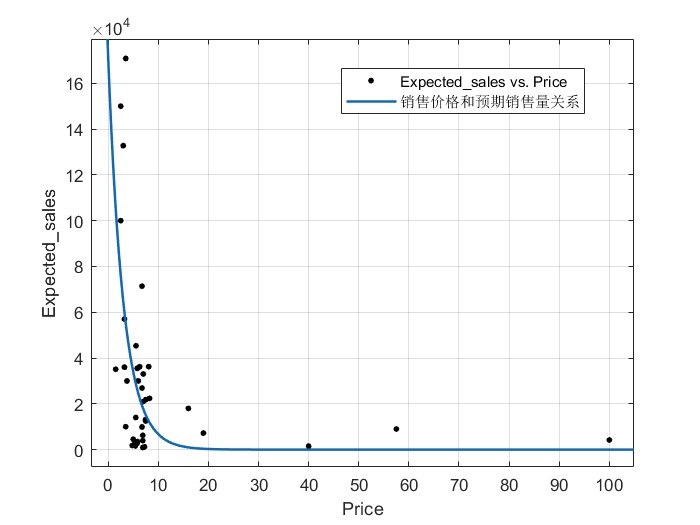
\includegraphics[height=0.2\textheight]{销售量和销售价格}
		\subcaption{预期销售量与销售价格拟合曲线}
	\end{minipage}
	\begin{minipage}[c]{0.48\textwidth}
		\centering
		
\includegraphics[height=0.2\textheight]{111}
		\subcaption{拟合统计量}
	\end{minipage}
\end{figure}

其中调整后$r$方为0.31,说明预期销售量与销售价格之间有一定的\textbf{负相关性},根据实际经济意义,我们界定当某类作物售价提高1$\%$时,其预期销售量应当降低0.3$\%$。
\begin{itemize}
	\item \textbf{销售价格与销售成本拟合}
\end{itemize}
\begin{figure}[H]
	\centering
	\begin{minipage}[c]{0.48\textwidth}
		\centering
		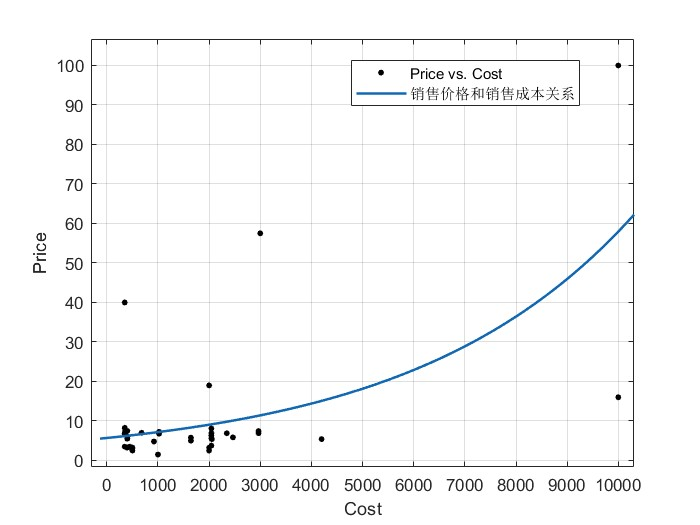
\includegraphics[height=0.2\textheight]{销售价格和成本}
		\subcaption{销售价格与销售成本拟合曲线}
	\end{minipage}
	\begin{minipage}[c]{0.48\textwidth}
		\centering
		
\includegraphics[height=0.2\textheight]{222}
		\subcaption{拟合统计量}
	\end{minipage}
\end{figure}

其中调整后$r$方为0.38,说明销售价格与销售成本之间有一定的\textbf{正相关性},根据实际经济意义,我们界定当某类作物成本提高1\%时,其销售价格应当上升0.3\%。

\begin{itemize}
	\item \textbf{预期销售量和销售成本拟合}
\end{itemize}
\begin{figure}[H]
	\centering
	\begin{minipage}[c]{0.48\textwidth}
		\centering
		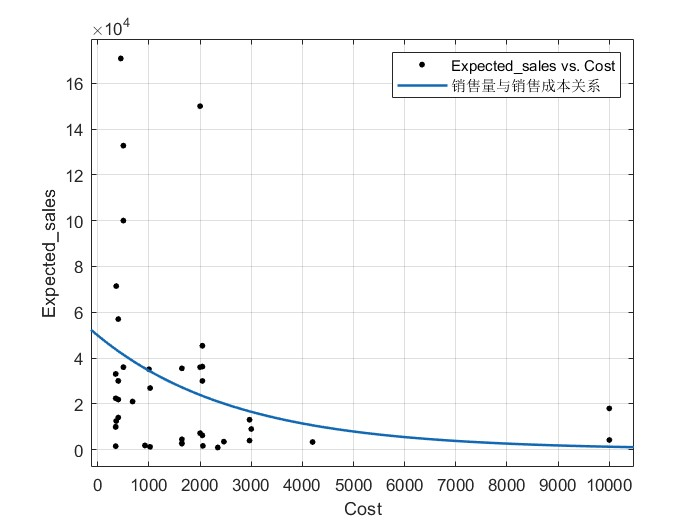
\includegraphics[height=0.2\textheight]{销量和成本}
		\subcaption{预期销售量和销售成本拟合曲线}
	\end{minipage}
	\begin{minipage}[c]{0.48\textwidth}
		\centering
		
\includegraphics[height=0.2\textheight]{333}
		\subcaption{拟合统计量}
	\end{minipage}
\end{figure}

其中调整后$r$方仅为0.04,说明销售价格和销售成本之间\textbf{几乎没有相关性},在计算由关联性产生的影响的时候可以忽略不记。
\subsection{模拟数据与求解}
我们设定,在每年由气候,市场等因素产生的不确定性对农作物各项数据发生波动之后,由于农作物的替代性与各项数据的关联性,还应当对再次数据进行调整,其调整幅度如上文所示,按照现实经济意义,其具体顺序步骤如下:
\begin{enumerate}
	\item 当某类作物成本提高1\%时,其销售价格应当上升0.3\%
	\item 当某类作物售价提高1\%时,其预期销售量应当降低0.3\%
	\item 当组内一类作物售价上涨1\%,其余作物销售量上涨0.5\%
\end{enumerate}

考虑到市场在一年内,售价,成本,销量并不能做出及时反应,只考虑对其做一次计算,不考虑循环计算。在每年进行完由不确定性带来的各项数据波动之后,再由其波动大小通过上述步骤进行二次波动计算,从而得到更加真实的农产品各项数据。



\subsection{模型的建立}
为了评价收益的经济性,我们引入经济指标$D$,来评价一种农作物表售价、成本,销量之间的经济性:
\begin{equation}
D_i=\omega _1\times \sum_{t=1}^2{{Cost^k}_{mjt}}+\omega _2\times \sum_{t=1}^2{{Price^k}_{mt}\times {PSale^k}_{mjt}}
\end{equation}

其中

$\omega _1=-\frac{\sum_{t=1}^2{{Cost^k}_{mjt}}}{\sum_{m=1}^{41}{\sum_{t=1}^2{{Cost^k}_{mjt}}}},\omega _2=\frac{\sum_{t=1}^2{{Price^k}_{mt}\times {PSale^k}_{mjt}}}{\sum_{m=1}^{41}{\sum_{t=1}^2{{Price^k}_{mt}\times {PSale^k}_{mjt}}}}
$

$D_i$越大,表示某种作物经济性越好。

则我们有如下目标函数

\begin{align}
	\max \quad P &= \sum_{k=1}^7 \sum_{t=1}^2 \sum_{j=1}^{54} \sum_{i=1}^{41} \left( {PSale^k}_{ijt} \times {Price^k}_{it} - {Cost^k}_{ijt} \right) \times {X^k}_{ijt} \times {Y^k}_{ijt} \\
	\max \quad D &= \frac{\sum_{i=1}^{41} D_i \times \nu_i}{\sum_{i=1}^{41} D_i}, \quad \nu_i = \frac{\sum_{t=1}^2 {PSale^k}_{mjt}}{\sum_{m=1}^{41} \sum_{t=1}^2 {PSale^k}_{mjt}}
\end{align}
同时有如下约束:
\begin{equation}
	\left\{ \begin{array}{c}
		\begin{array}{l}
			\sum_{i=17}^{41}{\sum_{j=1}^{26}{\sum_{k=1}^7{\sum_{t=1}^2{Y_{ijt}^{k}=0}}}}\\
			\sum_{i=1}^{15}{\sum_{j=27}^{34}{\sum_{k=1}^7{\sum_{t=1}^2{Y_{ijt}^{k}=0}}}}\\
			\sum_{i=1}^{15}{\sum_{j=35}^{54}{\sum_{k=1}^7{\sum_{t=1}^2{{Y^k}_{ijt}=0}}}}\\
			\sum_{i=1}^{16}{\sum_{j=51}^{54}{\sum_{k=1}^7{\sum_{t=1}^2{{Y^k}_{ijt}=0}}}}\\
		\end{array}\\
		\sum_{i=38}^{41}{\sum_{j=51}^{54}{\sum_{k=1}^7{\sum_{t=1}^2{{Y^k}_{ijt}=0}}}}\\
		\sum_{i=1}^{16}{\sum_{j=1}^{26}{\sum_{k=1}^7{{Y^k}_{ij2}=0}}}\\
		\sum_{j=27}^{34}{\sum_{k=1}^7{{Y^k}_{1jt}=0}}\\
		{Y^k}_{ijt}+{Y^k}_{ij\left( t+1 \right)}\le 1\left( \text{其中}1\leqslant i\leqslant 5 \right)\\
		{X^k}_{ijt}\times {Y^k}_{ijt}\geqslant 0.2\times Area_j\times {Y^k}_{ijt}\\
		\sum_{t=n}^{n+5}{{Y^k}_{ijt}}\geqslant 1(n=1,2\cdots ,9)\\
	\end{array} \right. 
\end{equation}

\subsection{基于多目标遗传算法的最优化求解模型构建}

由于本问决策变量中既含有0-1变量又含有连续变量,传统遗传算法
的性能较差,需要使用混合编码和多目标规划的优化算法。本文采用\textbf{多目标遗传算法}
NSGA-II,并对其加以改进。相对于传统的多目标遗传算法,NSGA-II引入了\textbf{非支配排
序}技术,能够将个体按照非支配性进行分级,保留多个非支配解,找到更多的高质量解,

求得
\begin{equation}
	max \quad P=37680766.4 \quad max \quad D=0.7164
\end{equation}
\begin{thebibliography}{9}%宽度9
    \bibitem[1]{mathematical-modeling} 曹军,张加龙,肖庆琳,等.基于随机森林和蒙特卡洛的高山松地上碳储量估测及不确定性分析[J].林业科学研究,2023,36(05):131-139.
    \bibitem[2]{mathematical-modeling}
    全国大学生数学建模竞赛论文格式规范 (2020 年 8 月 25 日修改).
     \bibitem[3] {mathematical-modeling}游和远,张津榕,夏舒怡.面向碳排放效率的多目标土地利用结构与布局优化研究——以杭州市萧山区为例[J].中国土地科学,2023,37(06):74-83.
      \bibitem[4]{mathematical-modeling} 胡丹青,赵为华.基于遗传算法的多结构变点检测及其应用[J].统计与决策,2022,38(06):21-25.DOI:10.13546/j.cnki.tjyjc.2022.06.004.
\end{thebibliography}

\newpage
%附录
\begin{appendices}


\section{蔬菜类作物聚类}
\begin{longtable}{|c|c|c|c|}
	\caption{蔬菜类作物聚类}  \\
	\hline
	作物编号 & 作物名称 & 类别 & 中心距离  \\
	\hline
	\endfirsthead
	
	\hline
	作物编号 & 作物名称 & 类别 & 中心距离  \\
	\hline
	\endhead
	
	\hline
	\endfoot
	
	\hline
	\endlastfoot
	
	17 & 豇豆 & 1 & 1.642 \\
	18 & 刀豆 & 1 & 0.142 \\
	19 & 芸豆 & 1 & 0.358 \\
	20 & 土豆 & 2 & 0.078 \\
	21 & 西红柿 & 1 & 0.358 \\
	22 & 茄子 & 1 & 0.358 \\
	23 & 菠菜 & 1 & 0.558 \\
	24 & 青椒 & 2 & 0.922 \\
	25 & 菜花 & 1 & 0.358 \\
	26 & 包菜 & 1 & 0.142 \\
	27 & 油麦菜 & 2 & 0.922 \\
	28 & 小青菜 & 1 & 0.358 \\
	29 & 黄瓜 & 1 & 0.642 \\
	30 & 生菜 & 1 & 0.858 \\
	31 & 辣椒 & 1 & 0.642 \\
	32 & 空心菜 & 2 & 0.078 \\
	33 & 黄心菜 & 2 & 0.922 \\
	34 & 芹菜 & 2 & 0.122 \\
	35 & 大白菜 & 2 & 1.078 \\
	36 & 白萝卜 & 2 & 1.078 \\
	37 & 红萝卜 & 2 & 0.578 \\
\end{longtable}
\section{遗传算法--matlab 源程序}

\begin{lstlisting}[language=matlab]
clc,clear,close all;
options = optimoptions('ga', ...
'PopulationSize', 150, ...          % 增加种群规模
'CrossoverFraction', 0.8, ...
'FunctionTolerance', 1e-6, ...
'MaxGenerations', 50, ...            % 增加最大代数
'EliteCount', 5, ...                 % 增加精英个体数量
'Display', 'iter', ...
'ConstraintTolerance', 1e-6,...
'SelectionFcn', @selectiontournament,...
'CrossoverFcn', @crossoversinglepoint);% 使用单点交叉 );% 使用锦标赛选择);
% 'MutationFcn', {@mutationadaptfeasible, 0.2}); % 增加变异率
% 'CrossoverFcn', @crossoversinglepoint);% 使用单点交叉 
%% 导入数据
load danweicb.mat
load shoujia1.mat      %单位成本
load shoujia2.mat      
load muchang1.mat       %亩产量
load muchang2.mat 
load muchang_j.mat
load Area.mat          %面积
load neng1.mat          %能种
load neng2.mat
load area1.mat
load area2.mat
load xiaoliang.mat     %销量
i = 41; %41种作物
j = 54; %54块土地
T = 2;  %3年 6个季度
prob = optimproblem("ObjectiveSense",'max');
neng = cat(3,neng1,neng2);
area = cat(3,area1,area2);
shoujia = cat(3,shoujia1,shoujia2);
muchang = cat(3,muchang1,muchang2);
%% 优化变量定义
X = optimvar("X",i,j,T,'Type','continuous','LowerBound',0,'UpperBound',area);
Y = optimvar("Y",i,j,T,'Type','integer','LowerBound',0,'UpperBound',neng);
%% 目标函数
X_A = sum(X(:,1:6,:),2);    % 平旱地类型
X_B = sum(X(:,7:20,:),2);   % 梯田   
X_C = sum(X(:,21:26,:),2);  % 山坡地
X_D = sum(X(:,27:34,:),2);  % 水浇地
X_E = sum(X(:,35:50,:),2);  % 普通大棚
X_F = sum(X(:,51:54,:),2);  % 智慧大棚
X_type = [X_A X_B X_C X_D X_E X_F];%土地类型总矩阵
%决策变量土地汇总
Y_j = [sum(Y(:,1:6,:),2) sum(Y(:,7:20,:),2) sum(Y(:,21:26,:),2) ...
sum(Y(:,27:34,:),2) sum(Y(:,35:50,:),2) sum(Y(:,51:54,:),2)];
shouru = sum(X .* neng .* shoujia .*muchang .*Y,'all');
chenbeng = sum(danweicb(:,:,1:2) .* X_type,'all');
prob.Objective = shouru - chenbeng ;
%% 约束条件
cons2 = [];
cons3 = [];
%% 面积约束
expandedArea = repmat(Area, 1, 1, T);
logicalCons = sum(X) <= expandedArea;
cons1 = logicalCons(:)';
%% 不能重复约束
for m=1:41
m
for n=1:54
cons2 = [Y(m,n,1)+Y(m,n,2)<=1,cons2];
end
end
%% 年连续约束
load Y_last.mat
for m=1:15
for n=1:26
cons3 = [Y(m,n,1) + Y_last(m,n,1)<=1,cons3];
end
end
m=16;
for n=27:34
cons3 = [Y(m,n,1) + Y_last(m,n,1)<=1,cons3];
end
for m=17:34
for n =27:50
cons3 = [Y(m,n,1) + Y_last(m,n,1)<=1,cons3];
end
for n = 51:54
cons3 = [Y(m,n,1) + Y_last(m,n,2)<=1,cons3];
end
end
for m = 35:37
for n =27:34
cons3 = [Y(m,n,2) + Y_last(m,n,2)<=1,cons3];
end
end
for m = 38:41 
m
for n = 35:50
cons3 = [Y(m,n,2) + Y_last(m,n,1)<=1,cons3];
end
end
%% 销量约束
chang = sum(X_type  .* muchang_j(:,:,1:2),2);
yueshu = squeeze(chang) <= xiaoliang;
cons4 = yueshu(:)';
%%
prob.Constraints.con1=cons1;
prob.Constraints.con2=cons2;
prob.Constraints.con3=cons3;
prob.Constraints.con4=cons4;
[sol,fval] = solve(prob,'Options',options);
writematrix([sol.Y(:,:,1),sol.Y(:,:,2)],"01_24.xlsx","WriteMode","overwrite");
writematrix([sol.X(:,:,1),sol.X(:,:,2)],"Area_24.xlsx","WriteMode","overwrite");
Y_last = sol.Y;
save("Y_last.mat","Y_last");
% save("nian30.mat");
 \end{lstlisting}

 
\end{appendices}

\end{document} 